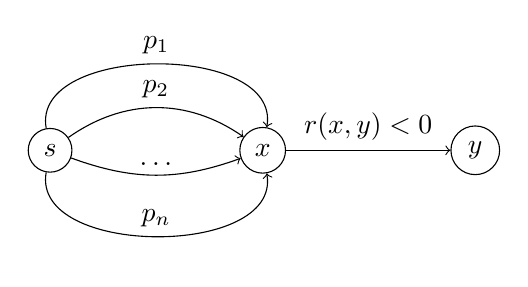
\begin{tikzpicture}[scale=0.9,state/.style={draw, circle, fill=none,text centered, text=black}]
    \node[state] (s) at (0, 0) {$s$};
    \node[state] (x) at (3, 0) {$x$};
    \node[state] (y) at (6, 0) {$y$};

    \draw [->] (x) -- node[anchor=south] {$ r(x,y) < 0 $} (y);

    \draw [->] (s) edge[bend right=-100] node[anchor=south] {$ p_1 $} (x);
    \draw [->] (s) edge[bend right=-35] node[anchor=south] {$ p_2 $} (x);
    \draw [->] (s) edge[bend right=20] node[anchor=south] {$ \dots $} (x);
    \draw [->] (s) edge[bend right=100] node[anchor=south] {$ p_n $} (x);
\end{tikzpicture}
